\section{Datasets}

There are a lot of 2D image datasets available for various purposes. Below is a list of some of the most popular:

\begin{itemize}
    \item \textbf{PASCAL Visual Object Classes (VOC)} is a dataset for object detection, segmentation, and classification. For the segmentation task, there are 21 labeled object classes and pixels are labeled as background if they do not belong to any of these classes. The dataset is divided into two sets, training and validation, with 1,464 and 1,449 images, respectively. An example image from the dataset is shown in Figure \ref{fig:pascal_voc}.
    \begin{figure}[t]
        \centering
         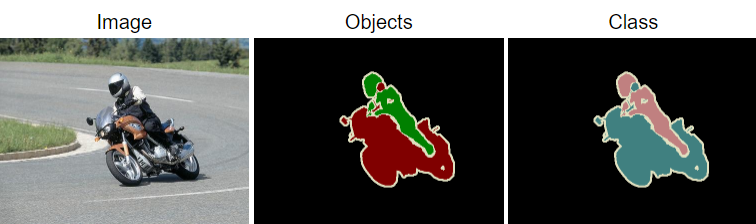
\includegraphics[width=0.8\linewidth]{images/pascal_voc.png}
      
         \caption{An example image from the PASCAL VOC dataset. From \cite{pascal_voc_dataset}}
         \label{fig:pascal_voc}
      \end{figure}
    \item \textbf{Cityscapes} contains a diverse set of stereo video sequences recorded in street scenes from 50 cities, with high-quality pixel-level annotation of 5,000 frames, in addition to a set of 20,000 weakly annotated frames. It includes semantic and dense pixel annotations of 30 classes, grouped into 8 categories — flat surfaces, humans, vehicles, constructions, objects, nature, sky, and void. An example image from the dataset is shown in Figure \ref{fig:cityscapes}.
    \begin{figure}[t]
        \centering
         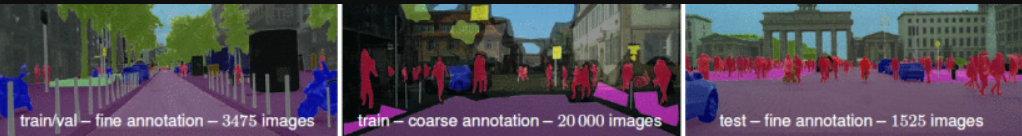
\includegraphics[width=0.8\linewidth]{images/cityscapes_example.png}
      
         \caption{An example image from the Cityscapes dataset. From \cite{7780719}}
         \label{fig:cityscapes}
      \end{figure}
\end{itemize}